\section{BOO}

\begin{frame}
\frametitle{BOO, FMO}
\begin{itemize}
	\item \small Aim high-precision, geometrically-shaped photons to tumors
\end{itemize}
	\begin{columns}[c]
		\begin{column}{.5\textwidth}			
			\centering
			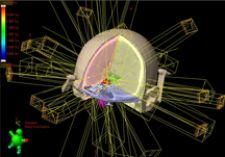
\includegraphics[width=\linewidth]{figures/boo-eclipse.jpg}
		\end{column}
		\-
		\begin{column}{0.5\textwidth}
			\centering
			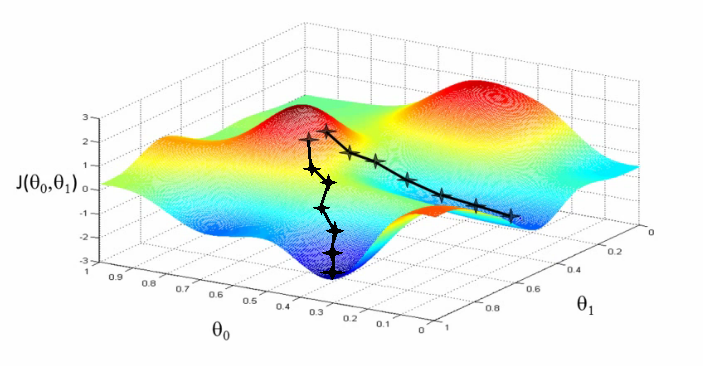
\includegraphics[width=\linewidth, height=.8\linewidth]{../Proposal/figures/nonconvex.png}
			\\
			\tiny Reprinted from David Shepard's AAPM Slides
		\end{column} 
	\end{columns} 
	%
	\begin{itemize}
		\item \small Beamlets from photons; optimal beam angles; FMO process $\rhd$ intensity modulation  
	\end{itemize}
\end{frame}

\begin{frame}
\frametitle{Existing Approaches}
\begin{itemize}
		\small
		\item Stochastic optimization approaches (SA, GA): ~\cite{ Bortfeld1993, Sodertrom1993,Pugachev2000,Pugachev02,Aleman08, Bertsimas2013}
		%
		\vspace{0.1in}
		%
		\item Gradient search:~\cite{Stein97, Craft2007, Bertsimas2013}
		%
		\vspace{0.1in}
		%
		\item Feature-based machine learning:~\cite{lu2006learning, li2010feasible}
		%
		\vspace{0.1in}
		%
		\item Mixed-integer LP, branch and cut, beam angle elimination algorithms: ~\cite{wang2003optimization, dsouza, lim2007optimization,Jia2011}
\end{itemize}
\end{frame}

\subsection{Proposal Two-Player}
\begin{frame}
\frametitle{An ADP + Monte-Carlo Evaluation Proposal}
\begin{itemize}
	\item \textbf{Context}: For $180$ discretized angles in a $5$ beam plan, there are $188,956,800,000$ possible search directions
	%
	\vspace{0.1in}
	%
	\item \textbf{Proposal}
	
	\begin{itemize}
		\item Monte-Carlo game planning strategy
		%
		\vspace{0.1in}
		%
		\item Deep neural network policy: map patients geometry to beam angles
		%
		\vspace{0.1in}
		%
		\item Refine accuracy of beams selection policy with fictitious self-play~[\cite{Heinrich}] 
	\end{itemize}
\end{itemize}
\end{frame}

\begin{frame}
\frametitle{State Representation: Network Input Plane}
\includegraphics[width=.85\columnwidth]{../../../BOO/figures/new_architecture.png}
\footnotetext{\tiny Net policy: produces a subjective probability distribution about a rational decision-making agent's preference for a \textit{lottery} (or \textit{value}) in an uncertain environment. 
	%It characterizes a  policy's belief about all relevant unknown factors at the current time step $k$ given a decision $u_k$. 
With new information, decision-maker's subjective probability distribution gets revised. Repeatedly sampling from this probability distribution enables the transition between episode contexts, \ie $\state_k \rightarrow \state_{k+1}$.}
\end{frame}

\frame{
	\frametitle{Two-Player Framework}
	\begin{itemize}
		\item Players base their decisions on a random event's outcome 			
		%
		\vspace{0.1in}
		%
			\item Guided by  a nonstationary Markovian policy set $\Pi^{p_i} =  \{\Pi^{p_1},  \Pi^{p_2}\}$ such that
			%
			\begin{itemize}
			%
			\item $\policy^{p_1} \in \{\pi^{p_1}_0, \pi^{p_1}_1, \ldots, \pi^{p_1}_{T}\} \subseteq \Pi^{p_1}$
			%
			\vspace{0.1in}
			%
			\item $\policy^{p_2} \in \{ \pi^{p_2}_0, \pi^{p_2}_1, \ldots , \pi^{p_2}_{T}\} \subseteq \Pi^{p_2}$
		\end{itemize}
	%
	\vspace{0.1in}
	%
	\item  \textbf{Stochastic action selection strategy} $\policy(\action|\state) :=\{\policy^{p_1}, \policy^{p_2}\}$ contain control sequences $\{\action^{p_1}_t\}_{0 \le t \le T}$ and $\{\action^{p_2}_t\}_{0 \le t \le T}$
	\end{itemize}
}

\begin{frame}
\frametitle{Cost-to-go}
%
\begin{itemize}
	\item Optimal \textbf{cost-to-go} value function for state %$\state$ in stage $t$, with horizon length $T$ 
	%
	\begin{align}
	V_t^*(\state) & = \inf_{\pi^{p_1} \in \Pi^{p_1}} \sup_{\pi^{p_2} \in \Pi^{p_2}} \bb{E}\left[\sum_{t=i}^{T-1} V_t(\state_0, f(\state_t, \pi^{p_1}, \pi^{p_2})) \right], \nonumber \\
	&	\qquad  \state \in \textbf{X}; \, V_T^*(\state) = 0, \, \, \forall \, \state \in \textbf{X}\nonumber
	\end{align}
	%
	\item Each player % bases its decision on a random event's outcome 
	generates a \textbf{mixed strategy} determined by \textbf{averaging the outcome} of individual plays
	%
	\item  Find optimal saddle point control pair $\{\action^{p^*_1}_t, \action^{p^*_2}_t\}$ % can be recursively obtained by %optimizing a state-action value cost, $\cost_t(\netstate, \action)$ 
	%
%	\begin{align}
%	V_t^*(\state_t, \policy^{p_1}_t, \policy^{p_2}_t) &= \min_{\policy^{p_1} \in \Pi^{p_1}} \max_{\policy^{p_2} \in \Pi^{p_2}} V^\star_t(\state_t, \policy^{p_1}, \policy^{p_2})   \\
%	%
%	\, & \quad \forall \, \state_t \in \mc{S}, \policy^{p_1} \in \Pi^{p_1}, \policy^{p_2} \in \Pi^{p_2}.
%	\end{align}
such that
\[
V^\star_{p_1} \le V_t^\star \le V^\star_{p_2} \quad \forall \,  \{\pi^{p_1}_t, \pi^{p_2}_t\}_{0 \le t\le T}.
\]
%where $V^\star_{p_i}$ are the respective optimal values for each player. 
\end{itemize}
\end{frame}

\subsection{Search}
\begin{frame}
\frametitle{Game Tree Simulation}
\begin{itemize}
	\item Network roll-out policy guides a tree's game, $\Gamma$, toward a \textit{best-first} set of  beam angle candidates
	%
	\vspace{0.1in}
	%
	\item Essentially, a sampling-based lookout algorithm 
	%
	\vspace{0.1in}
	%
	\begin{itemize}
		\item Focus on state space regions with least FMO score for beam angle combinations
		%
		\vspace{0.1in}
		%
		\item Lookout simulation steps: \textbf{Selection}; \textbf{Expansion};  \textbf{Simulation}; \textbf{Back-up}
		%
		\vspace{0.1in}
		%
		\item A `best move' for current beam block  selected, after each  iteration
	\end{itemize}  
\footnotetext{\tiny \textit{Selection}: from root node,  recursively apply child selection policy to navigate tree branches  until an expandable node is encountered. \textit{Expansion}:  iteratively add one or more children to the current node, based on the available move probabilities.
}
\end{itemize}
\end{frame}

\subsection{Fluence Map Optimization}
\begin{frame}
\frametitle{Fluence Map Optimization (FMO)}
\begin{itemize}
	\item Suppose $\voxtot$ is the total discretized $VOI$'s in a target volume
	%
	\vspace{0.1in}
	%
	\item Suppose $\beamlets_1 \cup \beamlets_2 \cup \ldots \cup \beamlets_n \subseteq \beamlets$ represents the partition subset of a  beam $\beamlets$
	%
	\vspace{0.1in}
	%
	\item Suppose further that $\dij(\beamangle_k)$ is the matrix that describes each dose influence, $d_i$.
	%
	\vspace{0.1in}
	%
%	\item  $\dij(\beamangle_k)$ delivered to a discretized voxel, $i$, in a volume of interest, $VOI_h \, (h = 1, \ldots, \voxtot)$, from a beam angle, $\beamangle_k$, $k \in \{1, \ldots, n\}$
%	%
%	\vspace{0.1in}
	%
	\item $\dij(\beamangle_k)$ is computed for each dose to voxel $i$ occupying a bixel, $j$, incident from a beam angle, $\beamangle_k$ at every $360^\circ/\varphi^\circ$. NB: $j \in \beamangle_k$
\end{itemize}
\end{frame}
%
\begin{frame}
\frametitle{The FMO Problem}
\begin{itemize}
\item Pre-calculated dose term:  $\Amat\primal = \{\sum_s\frac{w_s}{v_s} \dij^s \primal_s  \, | \, \dij^s \in \bb{R}^{n \times l}, n \gg l \}$%, which is a combination of the dose components that belong to OARs and those that belong to PTVs. 
%
\vspace{0.1in}
%
\item Find decision variable $\textbf{x}_j$ that maximizes dose to tumor, and  minimizes dose to critical structures and body tissues for all $k \in \{1, \ldots, n\}$
%
\vspace{0.1in}
%
\small \begin{align}
\small 
\min \frac{1}{v_s}\sum_{s \in \text{OARs}}  &\|(b_s - \underline{w}_s \dij^s \primal_s)_+ \|_2^2 + \frac{1}{v_s}\sum_{s \in \text{PTVs}}  \|(\bar{w}_s \dij^s \primal_s - b_s)_+\|_2^2 \nonumber \\
&\quad  \text{ subject to }  \textbf{x} \ge 0. \nonumber
\end{align}
%
\item Restated as
\[
\min \frac{1}{2}\|A \textbf{x} - \textbf{b}\|_2^2  \quad \text{ subject to }  x \ge 0.
\]
\end{itemize}
\end{frame}
%
\begin{frame}
\frametitle{FMO Lagrangian}
\begin{itemize}
\item  Lagrangian:
%
\[
L(\primal, \bm{\lambda}) = \frac{1}{2}\|A \textbf{x} - \textbf{b}\|_2^2 - \bm{\lambda}^T \primal.
\]
%\item Since we are solving a large scale problem, we use the ADMM algorithm
%
\item Introduce the auxiliary variable $\textbf{z}$, we have 
\begin{align}
\min_{\primal} \frac{1}{2}\|\Amat \primal - \textbf{b}\|_2^2,
\,\,\, \text{ subject to }  \admmvar = \primal, \,\, \admmvar \ge 0, \nonumber
\end{align}
\end{itemize}
\end{frame}


\begin{frame}
\frametitle{FMO Primal and Dual Updated}
\begin{itemize}
\item Solving the $\primal$ and $\admmvar$ sub-problems, we have
%
\tcb{
\begin{align}
\primal^{k+1} &= \left(\Amat^T\Amat + \rho \bm{I}\right)^{-1}\left(\Amat^T\bm{b}+ \rho \admmvar^k - \bm{\lambda}^k\right)  \nonumber \\
%\label{eq:admm_xupdate}
%
\admmvar^{k+1} &= S_{\bm{\lambda}/\rho}\left(\primal^{k+1} + \bm{\lambda}^k \right)%,
\nonumber
\end{align}
}{$\primal,\admmvar$-updates}
%
%
where $S_{\bm{\lambda}/\rho}(\tau) = (\primal - \bm{\lambda}/\rho)_+ - (-\tau - \bm{\lambda}/\rho)_+$, and %$\bm{\lambda}$ is updated as
%
\[
\bm{\lambda}^{k+1} = \bm{\lambda}^k - \gamma (\admmvar^{k+1} - \primal^{k+1}),
\]
with $\gamma$ as the step length controlling parameter.
\end{itemize}
\end{frame}

\subsection{Results}
\newcommand{\putdose}[2]{\includegraphics[width=#2\columnwidth, height=.45\columnwidth]{../../../BOO/figures/dvh_dose/#1}}
\newcommand{\dosewidth}{.5}

\newcommand{\putdvh}[2]{\includegraphics[width=#2\columnwidth, height=.42\columnwidth]{../../../BOO/figures/dvh_dose/#1}}
\newcommand{\dvhwidth}{.5}

\begin{frame}
\frametitle{Results: Dose Wash Plot}
\begin{table}[tb!]
	\centering
	\begin{tabular}{c@{}c@{}}
		%
		\putdose{case_007/dose.png}{\dosewidth} & \putdose{case_022/dose.png}{\dosewidth}
		%
	\end{tabular}
	\label{tbl:dose}
	%
\end{table}
\end{frame}


\begin{frame}
\frametitle{Results: Dose Wash}
\begin{table}[tb!]
\centering
\begin{tabular}{c@{}c@{}}
	%
	\putdose{case_075/dose.png}{\dosewidth} & \putdose{case_077/dose.png}{\dosewidth} 
	%
\end{tabular}
\label{tbl:dose_test}
%
\end{table}
\end{frame}

%\begin{frame}
%\frametitle{Results: Clinically Optimized DVH Curve}
%\begin{columns}[c]
%	\begin{column}{.5\textwidth}
%		\includegraphics[width=\linewidth]{../../../BOO/figures/clinic_plan.png}
%	\end{column}
%	\begin{column}{.5\textwidth}
%		\includegraphics[width=\linewidth]{../../../BOO/figures/dvh_dose/case_007/dvh.png}
%	\end{column}
%\end{columns}
%\end{frame}
%
%\begin{frame}
%\frametitle{Results: Deep BOO Optimized DVH Curve}
%\begin{columns}[c]
%	\begin{column}{.5\textwidth}
%		\includegraphics[width=\linewidth]{../../../BOO/figures/dvh_dose/case_022/dvh.png}
%	\end{column}
%\begin{column}{.5\textwidth}
%\includegraphics[width=\linewidth]{../../../BOO/figures/dvh_dose/case_075/dvh.png}
%\end{column}
%\end{columns}
%\end{frame}

\begin{frame}
\frametitle{Previously Proposed Future Work (Last Fall)}
\begin{itemize}
	\item Supervised Pretraining
	%
	\vspace{0.1in}
	%
	\begin{itemize}
		\item For example, PlanIQ or Column generation to eliminate plan quality gap and save training process time
		%	
		\vspace{0.1in}
		%
		\item Kalman filtering of predictions from neural network policy to obtain stable probabilities
	\end{itemize}
	%
	\item Robust policy improvement of pre-training angle predictions 
	%	
	\vspace{0.1in}
	%
	\begin{itemize}
		\item \eg Monte-Carlo Tree Search or Graph Convolutional Networks and guided tree search~[\cite{graphConvTreeSearch}].
	\end{itemize}
\end{itemize}
\end{frame}

\begin{frame}
\frametitle{Supervised Pre-Training of Deep BOO Policy}
\centering This page is left blank intentionally.
\end{frame}
